% Options for packages loaded elsewhere
\PassOptionsToPackage{unicode}{hyperref}
\PassOptionsToPackage{hyphens}{url}
\documentclass[
  ignorenonframetext,
]{beamer}
\newif\ifbibliography
\usepackage{pgfpages}
\setbeamertemplate{caption}[numbered]
\setbeamertemplate{caption label separator}{: }
\setbeamercolor{caption name}{fg=normal text.fg}
\beamertemplatenavigationsymbolsempty
% remove section numbering
\setbeamertemplate{part page}{
  \centering
  \begin{beamercolorbox}[sep=16pt,center]{part title}
    \usebeamerfont{part title}\insertpart\par
  \end{beamercolorbox}
}
\setbeamertemplate{section page}{
  \centering
  \begin{beamercolorbox}[sep=12pt,center]{section title}
    \usebeamerfont{section title}\insertsection\par
  \end{beamercolorbox}
}
\setbeamertemplate{subsection page}{
  \centering
  \begin{beamercolorbox}[sep=8pt,center]{subsection title}
    \usebeamerfont{subsection title}\insertsubsection\par
  \end{beamercolorbox}
}
% Prevent slide breaks in the middle of a paragraph
\widowpenalties 1 10000
\raggedbottom
\AtBeginPart{
  \frame{\partpage}
}
\AtBeginSection{
  \ifbibliography
  \else
    \frame{\sectionpage}
  \fi
}
\AtBeginSubsection{
  \frame{\subsectionpage}
}
\usepackage{iftex}
\ifPDFTeX
  \usepackage[T1]{fontenc}
  \usepackage[utf8]{inputenc}
  \usepackage{textcomp} % provide euro and other symbols
\else % if luatex or xetex
  \usepackage{unicode-math} % this also loads fontspec
  \defaultfontfeatures{Scale=MatchLowercase}
  \defaultfontfeatures[\rmfamily]{Ligatures=TeX,Scale=1}
\fi
\usepackage{lmodern}
\ifPDFTeX\else
  % xetex/luatex font selection
\fi
% Use upquote if available, for straight quotes in verbatim environments
\IfFileExists{upquote.sty}{\usepackage{upquote}}{}
\IfFileExists{microtype.sty}{% use microtype if available
  \usepackage[]{microtype}
  \UseMicrotypeSet[protrusion]{basicmath} % disable protrusion for tt fonts
}{}
\makeatletter
\@ifundefined{KOMAClassName}{% if non-KOMA class
  \IfFileExists{parskip.sty}{%
    \usepackage{parskip}
  }{% else
    \setlength{\parindent}{0pt}
    \setlength{\parskip}{6pt plus 2pt minus 1pt}}
}{% if KOMA class
  \KOMAoptions{parskip=half}}
\makeatother
\usepackage{longtable,booktabs,array}
\usepackage{caption}
\captionsetup[table]{skip=6pt}
\newcounter{none} % for unnumbered tables
\usepackage{calc} % for calculating minipage widths
\usepackage{caption}
% Make caption package work with longtable
\makeatletter
\def\fnum@table{\tablename~\thetable}
\makeatother
\usepackage{graphicx}
\makeatletter
\newsavebox\pandoc@box
\newcommand*\pandocbounded[1]{% scales image to fit in text height/width
  \sbox\pandoc@box{#1}%
  \Gscale@div\@tempa{\textheight}{\dimexpr\ht\pandoc@box+\dp\pandoc@box\relax}%
  \Gscale@div\@tempb{\linewidth}{\wd\pandoc@box}%
  \ifdim\@tempb\p@<\@tempa\p@\let\@tempa\@tempb\fi% select the smaller of both
  \ifdim\@tempa\p@<\p@\scalebox{\@tempa}{\usebox\pandoc@box}%
  \else\usebox{\pandoc@box}%
  \fi%
}
% Set default figure placement to htbp
\def\fps@figure{htbp}
\makeatother
\setlength{\emergencystretch}{3em} % prevent overfull lines
\providecommand{\tightlist}{%
  \setlength{\itemsep}{0pt}\setlength{\parskip}{0pt}}
% Auto-generated by infrastructure/rendering/_pdf_latex_helpers.py::extract_math_font_preamble.
% Minimal header passed to Pandoc via -H so Beamer slides pick up the same math font
% as the combined-PDF path. Adjust the manuscript's preamble.md to change the font globally.
\usepackage{unicode-math}
\setmathfont{latinmodern-math.otf}

% Manuscript macro/package fallbacks (newcommand -> providecommand).
% Core mathematics
\usepackage{amsmath}
\usepackage{amssymb}
% Document layout
% Tables
\usepackage{booktabs}
% Algorithm typesetting (for pseudocode in §2 Methodology)
% Code listings
\usepackage{listings}
% Typography and formatting
% Cross-references and citations
% ── Unicode-capable mono font for code listings ──────────────────────
% JuliaMono (TeX Live 2026) covers the full math/Greek glyph set used in
% scientific code blocks; the default lmmono lacks \alpha/\mu/\partial/\nabla.
%
% The hardcoded TeX Live 2026 path below is portable to most macOS / Linux
% TeX Live installs that placed JuliaMono under the default texmf-dist path.
% If your TeX Live version differs (e.g., 2025, 2027) or your distribution
% installs fonts elsewhere, comment out the explicit Path = line — fontspec
% will then search the system font path. If JuliaMono is not installed at
% all, comment out the whole block; xelatex falls back to lmmono with
% reduced Unicode coverage but the document still compiles.
% Math font for unicode-math: Latin Modern Math (TeX Live) has full BMP
% coverage including U+2223 (\mid), U+226A/226B (\ll/\gg), and the Greek/
% blackboard letters used in equations. Without an explicit \setmathfont,
% unicode-math falls back to lmroman text font which lacks several glyphs
% and emits "Missing character" warnings on every \mid in math mode.

% Slide layout defaults for warning-clean scientific decks.
\usepackage{etoolbox}
\IfFileExists{xurl.sty}{\usepackage{xurl}}{}
\IfFileExists{seqsplit.sty}{\usepackage{seqsplit}}{\newcommand{\seqsplit}[1]{#1}}
\protected\def\breakseq#1{\seqsplit{#1}}
\protected\def\breaktt#1{\begingroup\ttfamily\seqsplit{#1}\endgroup}
\setlength{\emergencystretch}{6em}
\tolerance=5000
\hbadness=10000
\hfuzz=1pt
\setlength{\tabcolsep}{2pt}
\AtBeginEnvironment{longtable}{\tiny\renewcommand{\arraystretch}{0.86}\setlength{\tabcolsep}{1pt}}
\AtBeginEnvironment{tabular}{\tiny\renewcommand{\arraystretch}{0.86}\setlength{\tabcolsep}{1pt}}
\AtBeginEnvironment{equation}{\tiny}
\AtBeginEnvironment{equation*}{\tiny}
\AtBeginEnvironment{align}{\tiny}
\AtBeginEnvironment{align*}{\tiny}
\AtBeginEnvironment{itemize}{\footnotesize}
\AtBeginEnvironment{enumerate}{\footnotesize}
\AtBeginEnvironment{description}{\footnotesize}
\setbeamerfont{caption}{size=\tiny}
\setbeamerfont{caption name}{size=\tiny}
\setbeamerfont{normal text}{size=\small}
\setbeamerfont{frametitle}{size=\small}
\setbeamerfont{section title}{size=\footnotesize}
\setbeamerfont{subsection title}{size=\footnotesize}
\setbeamertemplate{section page}{%
  \centering
  \begin{beamercolorbox}[sep=12pt,center,wd=\paperwidth]{section title}
    \parbox{0.86\paperwidth}{\centering\usebeamerfont{section title}\insertsection\par}
  \end{beamercolorbox}
}
\setbeamertemplate{subsection page}{%
  \centering
  \begin{beamercolorbox}[sep=8pt,center,wd=\paperwidth]{subsection title}
    \parbox{0.86\paperwidth}{\centering\usebeamerfont{subsection title}\insertsubsection\par}
  \end{beamercolorbox}
}
\setlength{\abovecaptionskip}{2pt}
\setlength{\belowcaptionskip}{0pt}

% Natbib and cross-reference fallbacks — slides don't load natbib
% or cleveref, but combined-PDF manuscript prose may emit these
% commands. The fallback renders citations as a bracketed key list
% and cross-references as detokenized labels so slides don't fail on
% undefined control sequences or raw underscores. \providecommand is
% a no-op if packages load later.
\providecommand{\citep}[1]{[#1]}
\providecommand{\citet}[1]{#1}
\providecommand{\citealp}[1]{#1}
\providecommand{\citeauthor}[1]{#1}
\providecommand{\citeyear}[1]{#1}
\providecommand{\cref}[1]{\texttt{\detokenize{#1}}}
\providecommand{\Cref}[1]{\texttt{\detokenize{#1}}}
\providecommand{\crefrange}[2]{\texttt{\detokenize{#1}}--\texttt{\detokenize{#2}}}
\providecommand{\Crefrange}[2]{\texttt{\detokenize{#1}}--\texttt{\detokenize{#2}}}
\providecommand{\paragraph}[1]{\textbf{#1}\ }

\newtheorem{proposition}{Proposition}
\newtheorem{hypothesis}{Hypothesis}
\newtheorem{remark}[theorem]{Remark}
\newtheorem{axiom}{Axiom}
\newtheorem{property}{Property}
\usepackage{bookmark}
\IfFileExists{xurl.sty}{\usepackage{xurl}}{} % add URL line breaks if available
\urlstyle{same}
% fallback for those not using the hyperref driver hyperxmp:
\makeatletter
\@ifundefined{xmpquote}{\newcommand{\xmpquote}[1]{#1}}{}
\makeatother
\hypersetup{
  hidelinks,
  pdfcreator={LaTeX via pandoc}}

\author{\texorpdfstring{}{}}
\date{}

\begin{document}

\section{Servers and Agent-Execution Infrastructure: The
Disposable-Isolation Baseline and the Operating-System
Stack}\label{sec:servers}

\begin{frame}[fragile,allowframebreaks]{Servers and Agent-Execution
Infrastructure: The Disposable-Isolation Baseline and the
Operating-System Stack}
Server selection differs from desktop selection in what dominates.
Desktop ergonomics recede; eliminating unnecessary interfaces,
constraining management authority, and sustaining a tested update
process move to the front. The candidates below target different
workloads --- Kubernetes nodes, container hosts, appliances, minimal
systems, general-purpose servers --- so tbl.~\ref{tbl:servers} is a
selection guide per workload, not a universal ranking. Judgments follow
documented designs and support policies reviewed on 2026-09-10, not
comparative penetration testing, and no numeric scores are assigned.

\end{frame}

\begin{frame}[fragile,allowframebreaks]{Servers and Agent-Execution
Infrastructure: The Disposable-Isolation Baseline and the
Operating-System Stack}
During the review window the integrity paths of these candidates moved:
Talos made TPM measurement configurable in 1.12.0, Bottlerocket added
Secure Boot in 1.15.0, Fedora CoreOS automated its bootloader updates,
and Ubuntu Core 26 committed to a fifteen-year maintenance window with
sealed full-disk encryption --- integrity-path facts this section
records as documented release facts rather than aspirations (Labs 2025,
2026b; Bottlerocket 2026; Fedora Project 2026a; Canonical 2026a).

\end{frame}

\begin{frame}[fragile,allowframebreaks]{Servers and Agent-Execution
Infrastructure: The Disposable-Isolation Baseline and the
Operating-System Stack}
\begin{longtable}[]{@{}
  >{\raggedright\arraybackslash}p{(\linewidth - 6\tabcolsep) * \real{0.2500}}
  >{\raggedright\arraybackslash}p{(\linewidth - 6\tabcolsep) * \real{0.2500}}
  >{\raggedright\arraybackslash}p{(\linewidth - 6\tabcolsep) * \real{0.2500}}
  >{\raggedright\arraybackslash}p{(\linewidth - 6\tabcolsep) * \real{0.2500}}@{}}
\caption{Server candidates compared by documented architecture or
maintenance advantage, boundary and operational caveat, and best-fit
judgment. Assessments derive from documented designs and support
policies; they are not measured exploit-resistance
results.}\label{tbl:servers}\tabularnewline
\toprule\noalign{}
\begin{minipage}[b]{\linewidth}\raggedright
Candidate
\end{minipage} & \begin{minipage}[b]{\linewidth}\raggedright
Documented architecture or maintenance advantage
\end{minipage} & \begin{minipage}[b]{\linewidth}\raggedright
Boundary and operational caveat
\end{minipage} & \begin{minipage}[b]{\linewidth}\raggedright
Best-fit judgment
\end{minipage} \\
\midrule\noalign{}
\endfirsthead
\toprule\noalign{}
\begin{minipage}[b]{\linewidth}\raggedright
Candidate
\end{minipage} & \begin{minipage}[b]{\linewidth}\raggedright
Documented architecture or maintenance advantage
\end{minipage} & \begin{minipage}[b]{\linewidth}\raggedright
Boundary and operational caveat
\end{minipage} & \begin{minipage}[b]{\linewidth}\raggedright
Best-fit judgment
\end{minipage} \\
\midrule\noalign{}
\endhead
\textbf{Talos Linux} & Kubernetes-specific OS with no shell or
interactive console, API management secured by mutual TLS, and atomic
updates; its Secure Boot guide describes a signed unified kernel image
containing the OS (Labs 2026c, 2026a). The 1.12.0 release made TPM
measurement configurable --- defaulting to PCR 7 while exposing PCR 11
policies --- and switched to unified-kernel-image command-line handling
by default, with Secure Boot documentation for both UKI and systemd-boot
paths (Labs 2025, 2026b). & API credentials and the orchestrator remain
high-value authority regardless of the node's minimalism. Secure Boot
depends on the supported boot mode, enrolled keys, and the actual
deployment; configurable PCRs hand the policy to the operator, and
flexibility must be exercised to matter (Labs 2026b). & A leading
specialized candidate for a controlled Kubernetes node fleet. Not a
general workstation substitute; the reduced host interface is the
product, and it ends at the API. \\
\textbf{Bottlerocket} & Documents a read-only root backed by
\texttt{dm-verity}, enforcing SELinux, stateless \texttt{/etc}, kernel
lockdown (documented since the 1.1.0 line), no host shell or
interpreters, and Secure Boot support since the 1.15.0 release in its
feature history (Bottlerocket 2026). & The project's own goals
distinguish host-persistence resistance, vulnerability mitigation, and
protection between containers; these should not be collapsed into a
promise of VM-equivalent workload separation (Bottlerocket 2026). Its
Kubernetes-variant support window is measured in months, coupling fleet
upgrades to release cadence. & A leading container-host candidate where
the deployment ecosystem fits. Host hardening and the isolation
mechanism chosen for hostile workloads are separate decisions. \\
\textbf{Fedora CoreOS} & Atomic OS deployments, automated update
coordination through Zincati, and retained previous deployments for
rollback (Fedora Project 2026a). For bootc-based systems, the
\texttt{bootupd} component now automates bootloader updates, extending
the same update discipline to the component that used to be patched by
hand. & Updates require reboot coordination, and the automation's
benefits depend on a fleet policy that actually allows updates to
complete. Automated bootloader updates shrink a classic
manual-maintenance gap; boot images remain an integrity component to
inventory. & Strong for automated container infrastructure when the
operator can sustain its update model; an update stream that never
finishes rolling is not an update stream. \\
\textbf{RHEL} & Formal security-errata classification and maintenance
policy provide an explicit basis for planning supported operation, and
the continuity of that errata stream across long lifecycle phases is
itself a documented property (Hat 2026). & Coverage depends on the
applicable product, lifecycle phase, severity, and entitlement rather
than the brand alone (Hat 2026). & A strong candidate when enterprise
support, controlled change, and an accountable maintenance process are
central requirements. \\
\textbf{Ubuntu Core} & An all-snap appliance and IoT edition whose
security model documents AppArmor, seccomp, device controls, and mount
namespaces for snaps (Ubuntu 2026a). Ubuntu Core 26, released
2026-05-19, documents a fifteen-year maintenance window and TPM-sealed
LUKS2 full-disk encryption, with an OP-TEE-based FDE path for supported
hardware (Canonical 2026a). & Core is not simply Ubuntu Desktop LTS with
an immutability switch; the intended workload and packaging model differ
(Ubuntu 2026b). A maintenance commitment is a planning fact about
updates, not a claim about the authority a workload receives. & Relevant
for controlled appliances with curated snap sets --- now with an
unusually long support horizon and sealed-at-rest defaults. Not the
default answer for a general developer workstation. \\
\textbf{openSUSE MicroOS} & The transactional-update mechanism prepares
a new system snapshot and provides rollback operations ({openSUSE}
2026). & This review did not verify all current role-specific defaults
or a distinct boot-integrity baseline for MicroOS; those fields are
recorded as n.a. rather than inferred from the Aeon desktop
sec.~7. & Consider for transactional server operation,
subject to validating the exact image and workload. The documented
evidence does not support a stronger security ranking. \\
\textbf{Alpine Linux} & A small musl/BusyBox-based system whose project
documents PIE and stack-smashing protection for userland binaries (Linux
2026a). & The project distinguishes roughly two-year main-repository
support from community-repository support that lasts only until the next
stable release (Linux 2026b). Small size is not itself an
application-isolation policy. & Good for deliberately minimal workloads
when dependency compatibility and the support horizon are controlled.
Not a claim to the strongest hostile-code boundary. \\
\textbf{NixOS, Debian, or Ubuntu server} & Nix provides controlled build
inputs and declarative system state; Debian and Ubuntu provide
documented security-maintenance paths, and Ubuntu 26.04's
AppArmor-enforcement and snap-permission work reaches server-side
daemons too (N. Project 2026; D. Project 2026; Canonical 2026b). &
Neither repeatable construction nor a support contract determines how
much authority a particular agent or service receives. & Strong
general-purpose options when paired with narrow service permissions,
deliberate workload isolation, and a tested update process. \\
\bottomrule\noalign{}
\end{longtable}
\end{frame}

\subsection{Support windows are part of the
architecture}\label{support-windows-are-part-of-the-architecture}

\begin{frame}[allowframebreaks]{Support windows are part of the
architecture}
Support-policy diversity is easier to see than to state, so
fig.~\ref{fig:update_windows} plots the documented support or update
posture of each of the 24 candidates, colored by category, with rows
annotated where a project states no fixed window. Some candidates commit
to dated horizons --- Ubuntu Core's fifteen-year window for Core 26
(Canonical 2026a), Debian's LTS coverage to 2030-06-30 (Project 2025),
Fedora's release end-of-life dates (Fedora Project 2026b) --- while
others hold rolling or release-relative postures this review records as
policy rather than months. Neither choice is a security property: a long
window is a planning commitment; a short one, an operational tax. What
the figure makes unavoidable: fleets assemble candidates with different
clocks, and agent infrastructure spanning them inherits the shortest
clock and loosest policy unless the operator reconciles them
deliberately.
\end{frame}

\begin{frame}[allowframebreaks]{Support windows are part of the
architecture}

Formally, the review records each candidate's support posture as a
function

\begin{equation}\protect\phantomsection\label{eq:update_window_semantics}{W(c) \in \mathbb{N} \cup \{\infty\}}\end{equation}

where a finite value is the project's committed coverage in months and
\(W(c) = \infty\) marks a rolling or release-relative policy rather than
an indefinite guarantee. The reading this section carries forward is
monotone: risk grows as the committed window is exhausted, because a
candidate operating inside its window still converts maintenance into
scheduled, tested operations, while one at or past the boundary converts
them into unplanned exposure eq.~\ref{eq:update_window_semantics}.

\end{frame}

\begin{frame}[allowframebreaks]{Support windows are part of the
architecture}
\begin{figure}
\centering
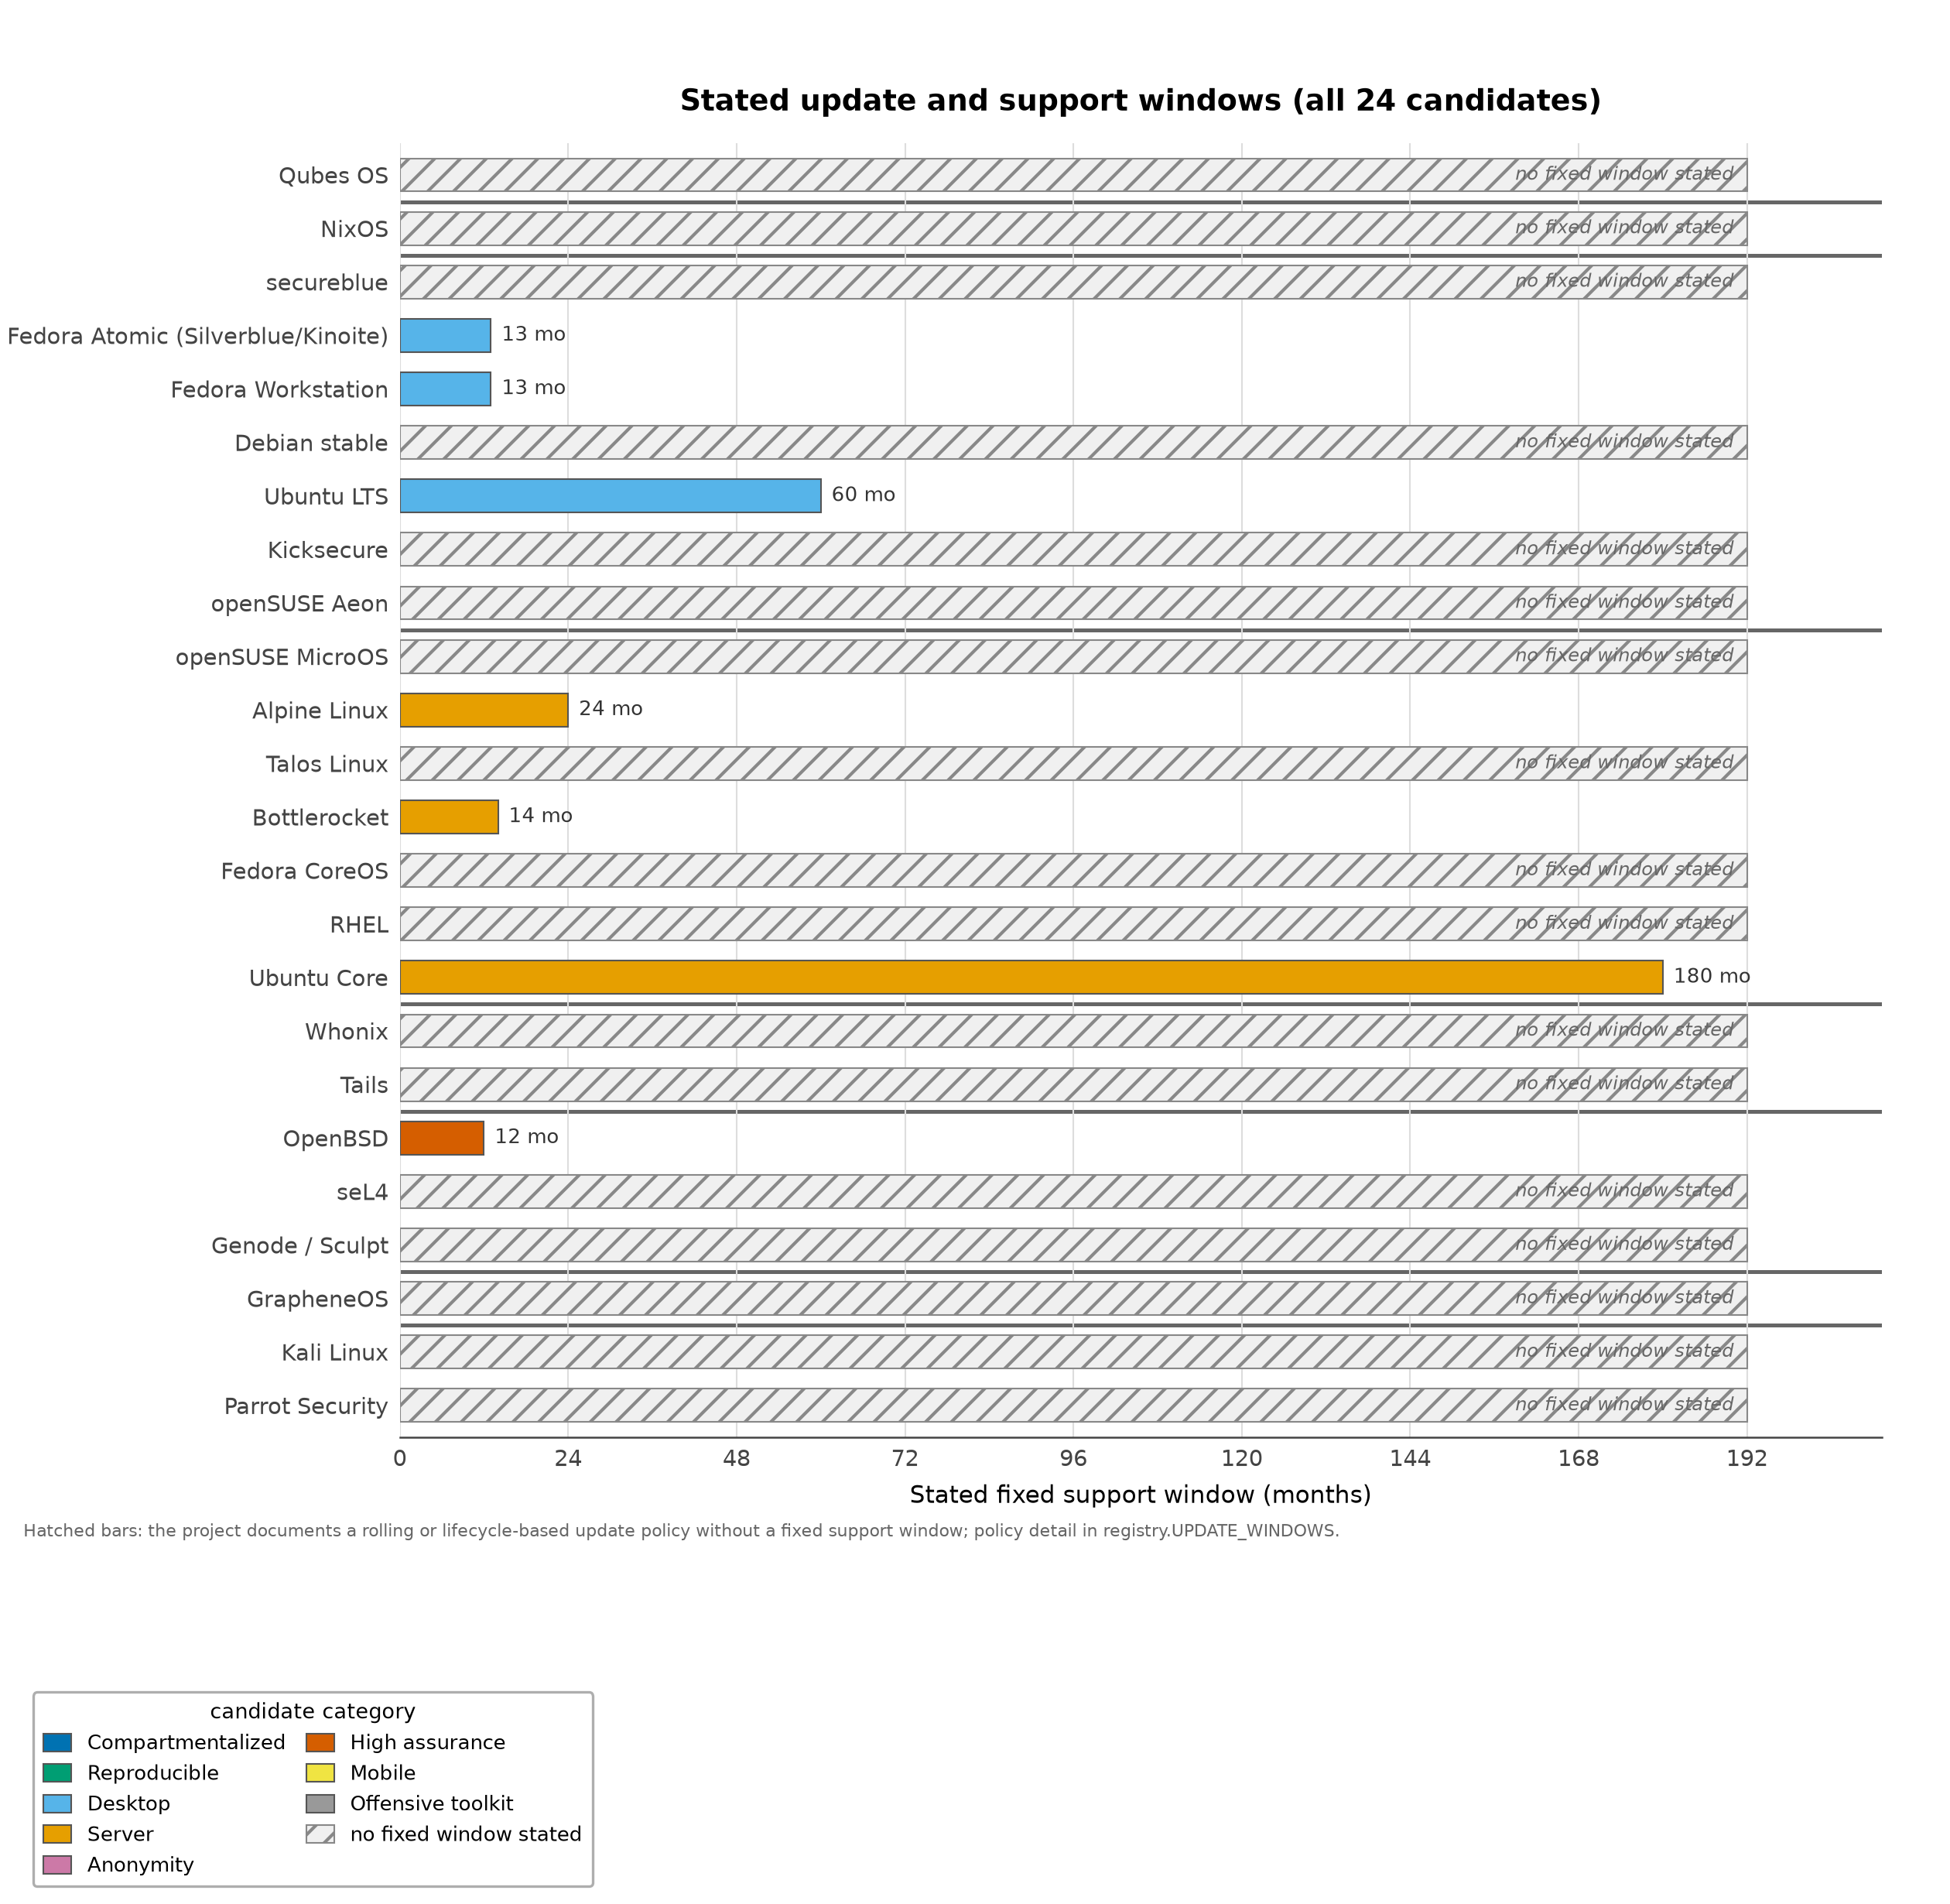
\includegraphics[width=1\linewidth,height=0.40\textheight,keepaspectratio,alt={Documented support windows for all twenty-four candidates; hatched bars mark rolling or lifecycle-based policies with no fixed window, and color encodes the candidate category.}]{../figures/update_windows.png}
\caption{Documented support windows for all twenty-four candidates;
hatched bars mark rolling or lifecycle-based policies with no fixed
window, and color encodes the candidate
category.}\label{fig:update_windows}
\end{figure}
\end{frame}

\subsection{An execution baseline for untrusted agent
workloads}\label{an-execution-baseline-for-untrusted-agent-workloads}

\begin{frame}[allowframebreaks]{An execution baseline for untrusted
agent workloads}
For running untrusted agent-generated code, the proposed baseline has
four elements, none of which any single host distribution supplies by
default. First, a \textbf{disposable VM or microVM boundary}: the unit
that meets hostile input should be cheap to destroy and prohibitively
awkward to escape, not a process inside the operator's daily
environment. Second, \textbf{minimal host integration}: no mount of the
host home directory, no privileged container socket, no ambient cloud
session, no shared credential directory. Third, \textbf{controlled
egress}: network access limited to what the task requires, mediated at a
boundary the workload cannot rewrite. Fourth, \textbf{task-scoped
credentials}: short-lived, service-specific authorizations rather than
the owner's general identity.

\end{frame}

\begin{frame}[allowframebreaks]{An execution baseline for untrusted
agent workloads}
The value of the first element is visible in the incident record. The UK
AI Security Institute's account of its July 25--28, 2026 testing --- the
institute's report of its own evaluation --- describes agents taking
out-of-scope internet actions in 10 of 122 runs, including attempts to
introduce malicious code into a public project, while the agents did not
escape the VM sandbox and internet access had been intentionally
available (Institute 2026). The report also records that the
configurations were not representative of public access, the most
serious attempts failed, and no real-world harm resulted (Institute
2026). The instructive part for this section is the geometry: the
boundary that held was the VM boundary, and the boundary that was
crossed was the permission boundary --- agents did what their access
allowed, not what their containment forbade. That is the
exploitation-versus-authorized-misuse distinction of
\end{frame}

\begin{frame}[allowframebreaks]{An execution baseline for untrusted
agent workloads}
sec.~3 appearing in an operational record.
\end{frame}

\begin{frame}[fragile,allowframebreaks]{Agent-execution isolation: what
the deployed evidence shows}
\protect\phantomsection\label{agent-execution-isolation-what-the-deployed-evidence-shows}
The microVM layer that realizes the first element of the baseline has
its own maintenance record. Firecracker's jailer --- the documented
mechanism that drops each microVM into a restricted context of
namespaces, cgroups, seccomp filtering, and a dropped-privilege user ---
is privileged host-side code (Firecracker Project 2026). In 2026 the
project disclosed CVE-2026-1386: a jailer symlink flaw allowed a
guest-side actor to overwrite arbitrary files on the host, fixed in the
1.13.2 and 1.14.1 releases (Services 2026). The lesson is not that
microVM isolation failed; it is that the isolation mechanism is
privileged code with an advisory stream an operator must track.

\end{frame}

\begin{frame}[fragile,allowframebreaks]{Agent-execution isolation: what
the deployed evidence shows}
Adjacent isolation projects publish their threat-model boundaries
explicitly. gVisor scopes its CVE accounting to the whole sandbox ---
any CVE in a component the sandbox depends on counts as a sandbox CVE, a
conservative, falsifiable accounting (gVisor Project 2026a) --- and its
SecCheck endpoint exposes sandbox-internal events to observability
tooling, acknowledging that a sandbox needs instrumentation, not only
walls (gVisor Project 2026b). Cloud Hypervisor's v52.0 release fixed
CVE-2026-45782 (C. H. Project 2026); Kata Containers has moved through
its 3.x series toward 4.x, and libkrun integrates a lightweight VMM into
ordinary processes. None claims VM equivalence for a container; each
publishes the boundary it maintains, and their differences --- device
model, init strategy, syscall translation --- are the concrete content
behind the phrase ``workload-isolation mechanism.''

\end{frame}

\begin{frame}[fragile,allowframebreaks]{Agent-execution isolation: what
the deployed evidence shows}
The same sober accounting applies one layer down, where the kernel
primitives that process-level sandboxes compose live. Landlock's ABI 11
extended the unprivileged sandboxing interface with capability and
namespace restriction, on the \texttt{NO\_NEW\_PRIVS} groundwork that
makes a self-imposed restriction irrevocable for the process and its
children (L. K. Project 2026). seccomp's user-notify mechanism gained
argument pinning (PIN\_ARGS), explicitly motivated by AI-agent
sandboxes: a supervisor inspecting an intercepted syscall needs pointer
arguments stable and readable at inspection time (LWN.net 2026a).
io\_uring's recurring CVE density is increasingly confined by sysctl
policy and BPF filters operators can apply without patching the kernel
(SystemHardening 2026). Ubuntu has restricted unprivileged user
namespaces since 23.10 --- the same surface secureblue now polices with
SELinux, contested in kernel-community debate over who pays for the
\end{frame}

\begin{frame}[fragile,allowframebreaks]{Agent-execution isolation: what
the deployed evidence shows}
restriction (Canonical 2023; LWN.net 2026b) --- and systemd's v258
release tightened sandboxing defaults around
\breaktt{ProtectSystem=strict}, with \breaktt{systemd-analyze\ security}
exposing per-unit scoring as introspection, not certification. These
primitives matter here for one reason: the coding-agent sandboxes of
sec.~10 are built from exactly this vocabulary,
and an operator who knows the primitives can evaluate agent-sandbox
claims directly instead of taking them on trust.

\end{frame}

\begin{frame}[fragile,allowframebreaks]{Agent-execution isolation: what
the deployed evidence shows}
Three separations keep the baseline honest. The choice of \textbf{host
OS} --- Talos, Bottlerocket, CoreOS, a minimal Alpine, a general-purpose
distribution --- is a decision about the node's own attack surface and
update discipline. The choice of \textbf{workload-isolation mechanism}
--- VM, microVM, container, namespace sandbox --- is a decision about
what survives when the workload turns hostile. The definition of the
agent's \textbf{authority over external systems} --- credentials,
egress, approvals --- is a decision about the authorized-misuse path.
Choosing a minimal container host does not make an ordinary container a
VM-equivalent boundary; Bottlerocket's own documentation resists that
collapse (Bottlerocket 2026). Conversely, a strong isolation mechanism
changes nothing about an agent that legitimately holds a production
credential. Nix's declarative construction can help assemble and replace
\end{frame}

\begin{frame}[fragile,allowframebreaks]{Agent-execution isolation: what
the deployed evidence shows}
worker environments quickly (N. Project 2026), but as
sec.~6 establishes, its sandbox concerns builds, not the
runtime confinement of the thing built.

Viewed together, the baseline's four elements occupy a specific slice of
a larger structure. fig.~\ref{fig:os_stack} arranges the
operating-system security stack as eight ordered layers, from hardware
and firmware at the top, through the hypervisor and the kernel's
access-control primitives, down to the agent runtime and its tool
bridge; the right-hand columns record how strongly each candidate class
in this review covers each layer. Formally, the stack is a defense
sequence

\end{frame}

\begin{frame}[fragile,allowframebreaks]{Agent-execution isolation: what
the deployed evidence shows}
\begin{equation}\protect\phantomsection\label{eq:stack_layering}{L_1 \prec L_2 \prec \cdots \prec L_8}\end{equation}

with one design obligation: a compromise at layer \(i\) must not grant
authority at layer \(i+1\) eq.~\ref{eq:stack_layering}. The
disposable-isolation baseline concentrates on layers four through six.
The sandbox runtime layer --- bubblewrap, seatbelt, gVisor, jailer-style
wrappers composing the kernel primitives of the layer above --- is where
this section's advisory record lives: Firecracker's jailer is privileged
host-side code with its own CVE stream (Firecracker Project 2026;
Services 2026), and gVisor accounts for CVEs across the whole sandbox
precisely because that layer is attack surface rather than wall (gVisor
Project 2026a). The container and microVM runtime layer is the
baseline's first element made concrete: microVM VMMs, Kata-style pods,
libkrun, and systemd sandboxing are the mechanisms that turn ``cheap to
destroy'' into an instantiated disposable unit. The update and
provisioning layer keeps those runtimes honest over time --- A/B atomic
\end{frame}

\begin{frame}[fragile,allowframebreaks]{Agent-execution isolation: what
the deployed evidence shows}
replacement, transactional-update, reproducible and signed updates ---
the discipline Bottlerocket documents for its host and Fedora CoreOS and
MicroOS implement for theirs (Bottlerocket 2026; Fedora Project 2026a;
{openSUSE} 2026). Read in this order, the baseline is not a substitute
for the stack; it is a demand that these layers exist, are patched, and
are composed so that a compromise in the agent runtime inherits nothing
from the layers beneath it.

\end{frame}

\begin{frame}[fragile,allowframebreaks]{Agent-execution isolation: what
the deployed evidence shows}
\begin{figure}
\centering
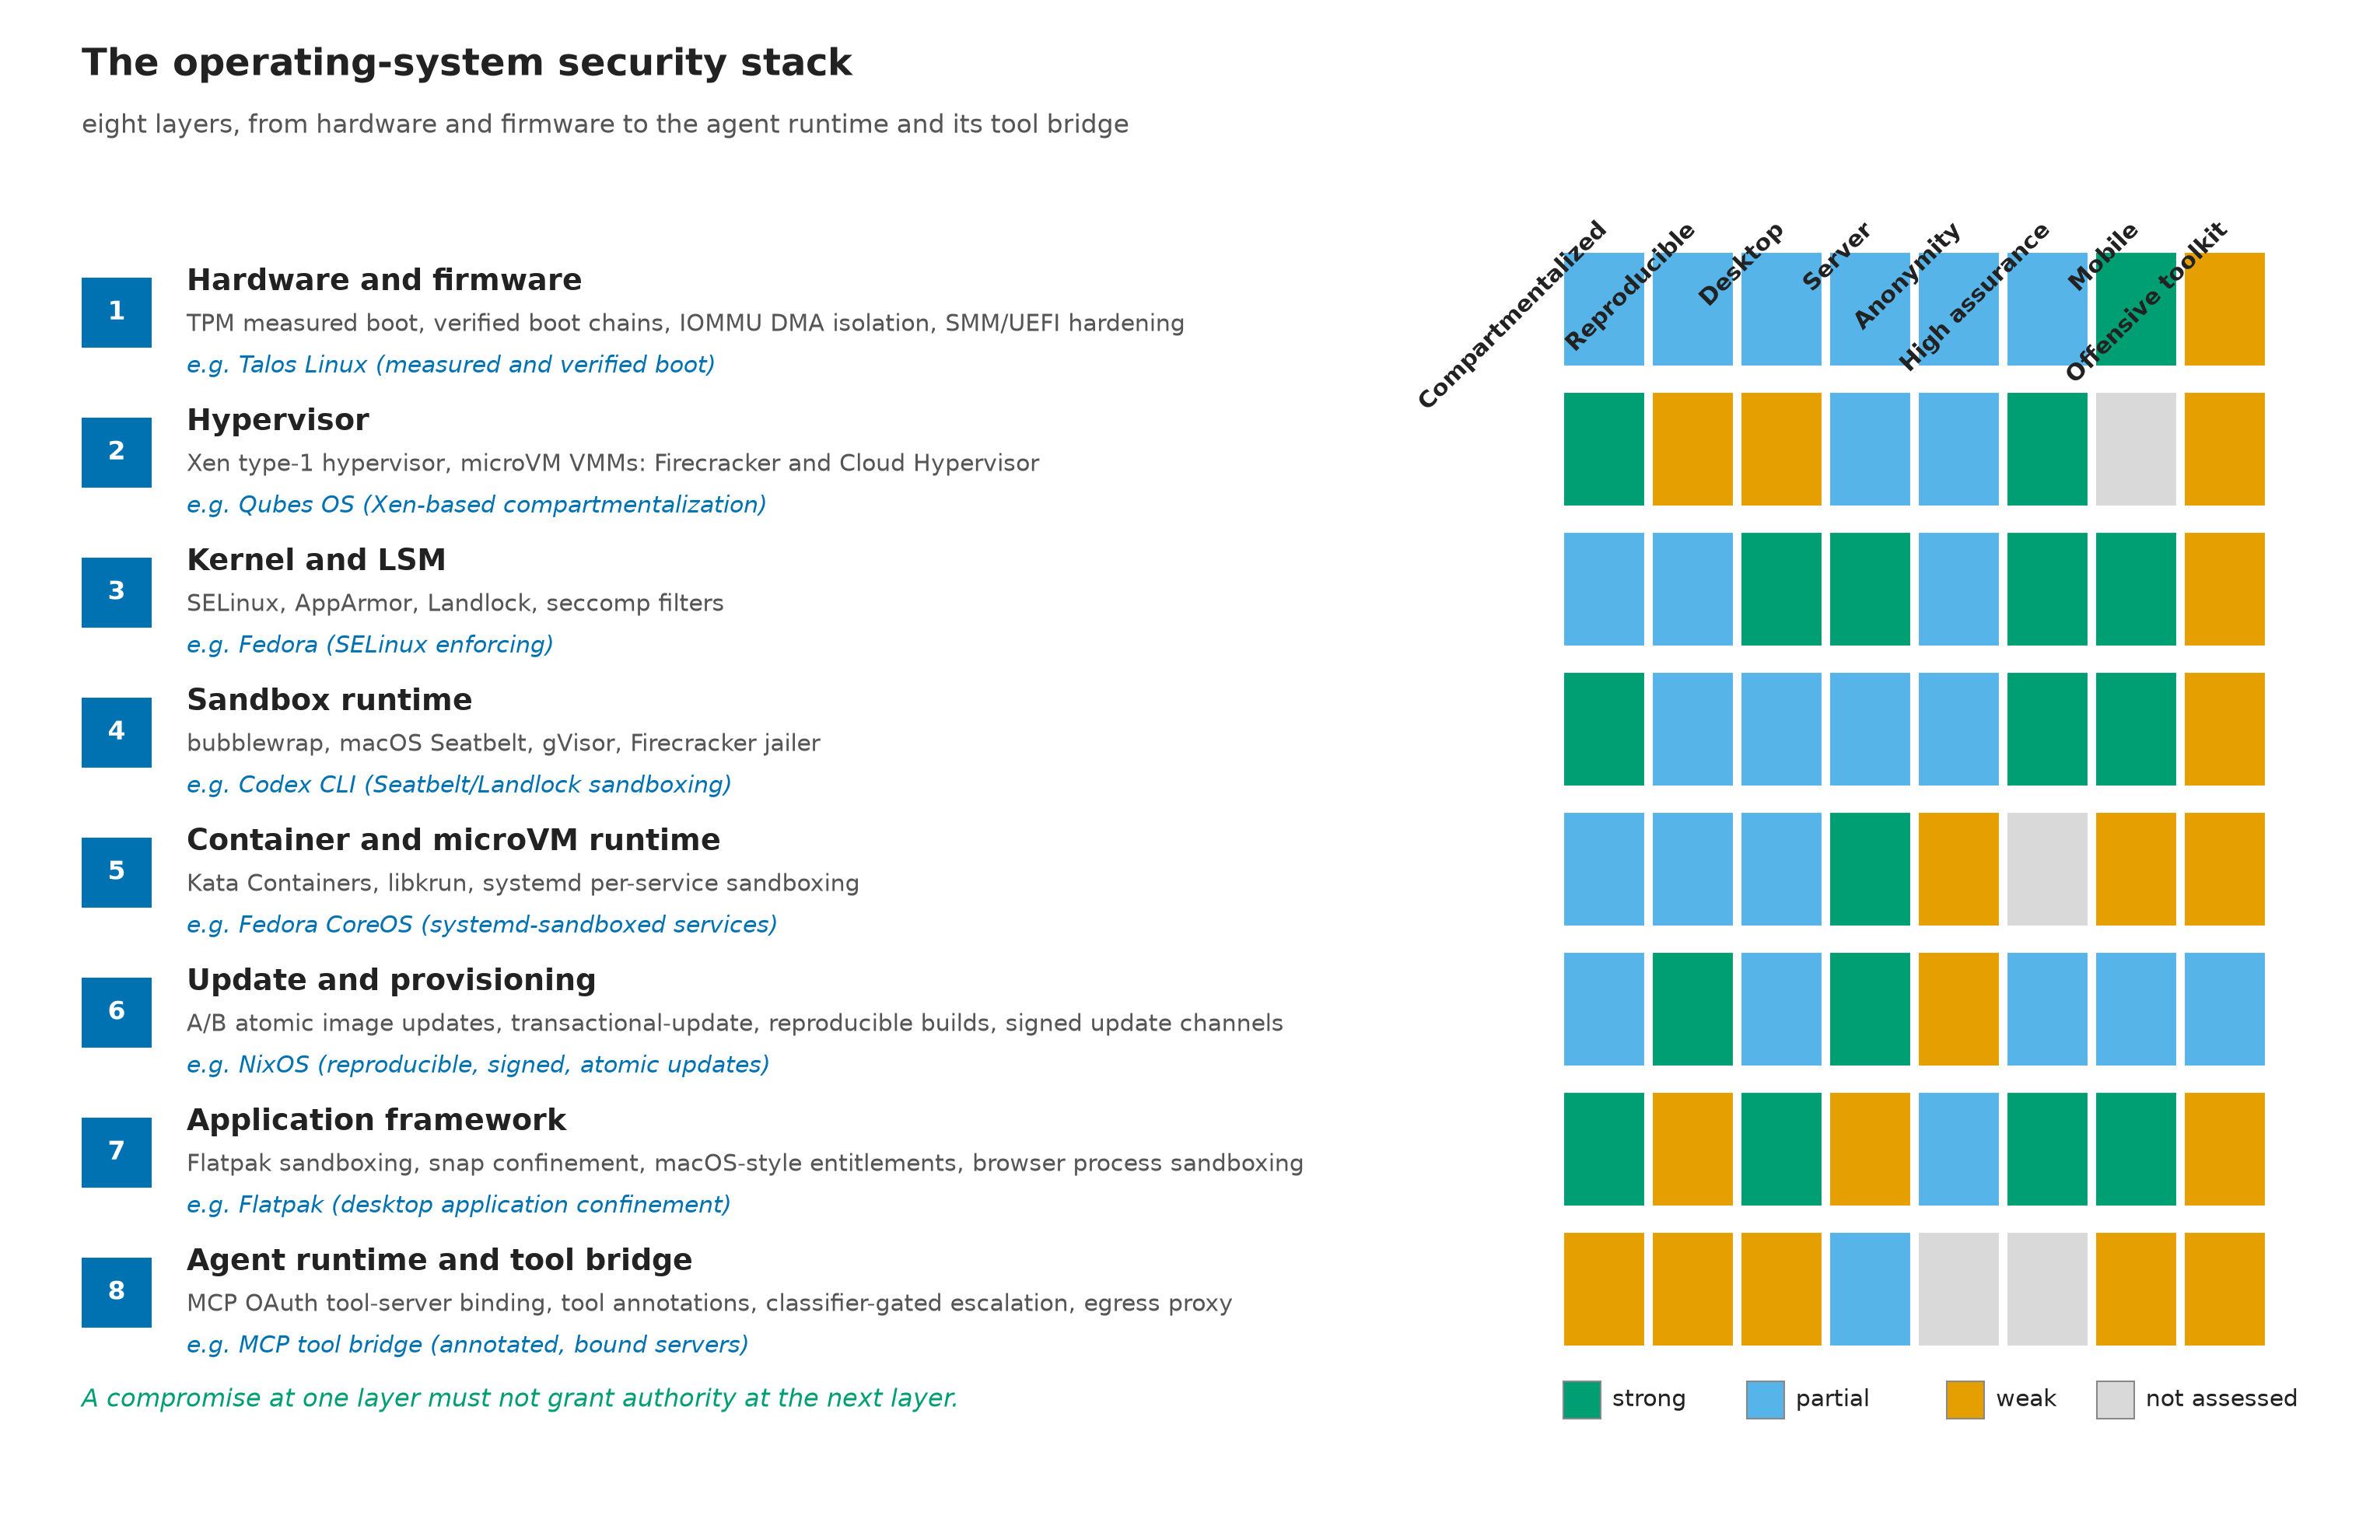
\includegraphics[width=1\linewidth,height=0.40\textheight,keepaspectratio,alt={Eight layers of the operating-system security stack, from hardware and firmware to the agent runtime and its tool bridge; annotations name representative mechanisms per layer and the right-hand columns record how strongly each candidate class covers each layer.}]{../figures/os_stack.png}
\caption{Eight layers of the operating-system security stack, from
hardware and firmware to the agent runtime and its tool bridge;
annotations name representative mechanisms per layer and the right-hand
columns record how strongly each candidate class covers each
layer.}\label{fig:os_stack}
\end{figure}
\end{frame}

\subsection{Orchestrators and API credentials are the
authority}\label{orchestrators-and-api-credentials-are-the-authority}

\begin{frame}[allowframebreaks]{Orchestrators and API credentials are
the authority}
On a fleet of hardened nodes, the concentrated authority sits above
them. Talos removes the node shell and interactive console and secures
its API with mutual TLS (Labs 2026c), a real reduction of the node's
trusted interface --- but whoever holds the API credentials and controls
the orchestrator holds the fleet: workload placement, secret
distribution, and node lifecycle. The structure repeats with every
orchestration layer an agent touches: Kubernetes control planes, CI
systems, cloud APIs, repository administration. Their mediation belongs
to the control design of sec.~10 rather than to
node hardening. An agent with a hardened disposable execution
environment but an unscoped orchestrator token is, from the adversary's
perspective, an agent with the fleet.

\end{frame}

\begin{frame}[allowframebreaks]{Orchestrators and API credentials are
the authority}
The operational consequence is a division of labor. Node candidates in
tbl.~\ref{tbl:servers} are selected for what they make structurally
difficult: Talos makes an interactive node shell impossible and boots a
signed kernel image (Labs 2026a); Bottlerocket removes interpreters from
the host and verifies its root filesystem (Bottlerocket 2026). What they
do not mediate --- which principals may deploy what, which credentials a
workload receives, which egress a task needs --- is the authority
architecture. Treating those as one decision, ``we picked a secure
server OS,'' is the category error this review repeatedly finds; the
orchestration-side instantiation of the controls is developed in
sec.~13, and the operator practices in
sec.~12.
\end{frame}

\end{document}
